\documentclass{beamer}

\usepackage[utf8]{inputenc}
\usepackage[T1]{fontenc}
\usepackage[francais]{babel}
\usepackage{multimedia}
\usepackage{textcomp}

\usetheme{Darmstadt}
\usecolortheme{seahorse}

\usepackage{graphicx}

\AtBeginSection[]{
    \begin{frame}
        \frametitle{Plan}
        \tableofcontents[currentsection,hideothersubsections]
    \end{frame} 
}

\titlegraphic{
    \begin{columns}
        \column{.15\textwidth}
        
\includegraphics[width=\textwidth]{img/imag.eps}
        \column{.45\textwidth}
        
\includegraphics[width=\textwidth]{img/topSolid.eps}
    \end{columns}
}

\title{TopSolid Project}
\author{Ariane Lefebvre \and Pablo Coves}
\date{}

\begin{document}
\maketitle

\section{Introduction}
\subsection{Missler software}
\begin{frame}
    \begin{figure}
        
\includegraphics[width=.8\textwidth]{img/topSolid.jpg}
        \caption{TopSolid Galaxy}
        \label{TopSolid}
    \end{figure}
\end{frame}
\begin{frame}
    \begin{itemize}
        \item First CAD/CAM solution on PC's in the 80's.\\
            200 people, international resellers and around 25M of turnover.
        \item TopSolid products:
            \begin{itemize}
                \item General CAD/CAM:
                    Modeling, assembly, kinematic, drafting.
                    Turning, milling.
                \item Tooling CAD/CAM:
                    Mold design, progressive, transfer and stamping die design. 
                    EDM.
                \item Sheet metal CAD/CAM:
                    Sheet metal design, flat pattern computation. 
                    Punching and cutting.
            \end{itemize}
    \end{itemize}
\end{frame}
\subsection{Progressive die tool}
\begin{frame}
    \begin{columns}
        \column{.3\textwidth}
        \begin{itemize}
            \item Punch die.
            \item Blank holder.
            \item Metal strip.
            \item Die holder.
        \end{itemize}
        \column{.7\textwidth}
        \begin{figure}
            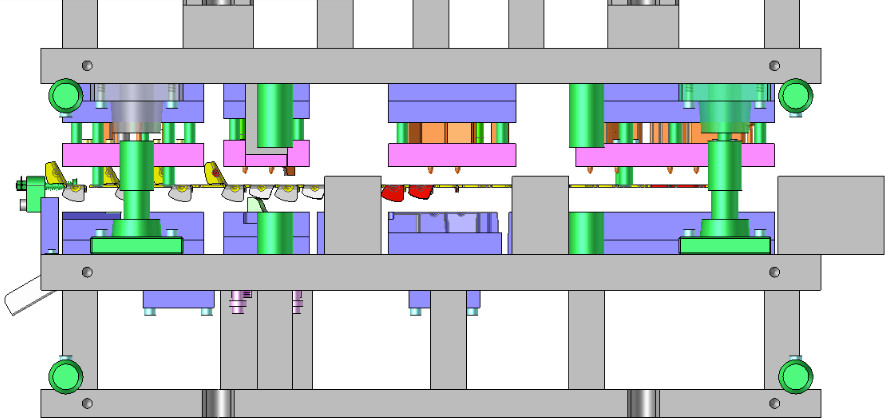
\includegraphics[width=\textwidth]{img/dieTool.jpg}
            \caption{Progressive die tool}
        \end{figure}
    \end{columns}
\end{frame}
\subsection{Basic operations}
\begin{frame}
    \begin{itemize}
        \item Cutting:\\
            Takes some parts of the initial material off.
        \item Bending:\\
            Creation of a formed feature by angular displacement of a sheet metal workpiece.
        \item Stamping:\\
            Change the shape of the initial material by pushing it strongly.
    \end{itemize}
\end{frame}
\section{Project content}
\subsection{Goal of the project}
\begin{frame}
    \frametitle{Bending simulation module}
    For specific productions in connector industry, the bending process needs to be simulated accurately in order to:
    \begin{itemize}
        \item Compute non intuitive trajectories of the free parts of the metal sheet during multiple bending process.
        \item Evaluate the spring back movement.
    \end{itemize}
\end{frame}
\subsection{Specifications}
\begin{frame}
    \begin{itemize}
        \item Bending simulation add-in.
        \item 2D representation.
        \item Sheet metal part geometry: constant thickness.
        \item Various punch die and punch holder shapes.
        \item Various material characteristics.
    \end{itemize}
\end{frame}
\begin{frame}
    \begin{columns}
        \column{.6\textwidth}
        A 2D representation of:
        \begin{itemize}
            \item \textbf{A die holder}: 
                A polygon which does not move over the time.
            \item \textbf{A blank holder}:
                A polygon that comes to fix a part of the metal sheet.
            \item \textbf{A punch die}:
                A polygon that we know the position over the time.
            \item \textbf{A metal strip}:
                With its fixed thickness, it is described by its neutral axis with well known characteristics.
        \end{itemize}
        \column{0.4\textwidth}
        \begin{figure}
            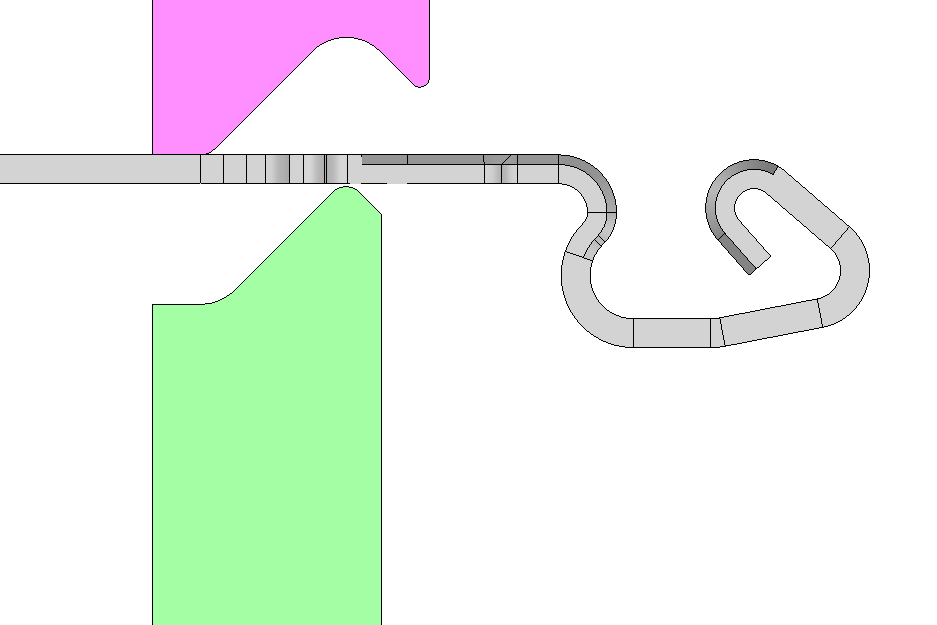
\includegraphics[width=\textwidth]{img/fibreNeutre.jpg}
            \caption{A 2D representation}
            \label{FibreNeudre}
        \end{figure}
    \end{columns}
\end{frame}
\subsection{Modelisation}
\begin{frame}
    In order to have a realistic representation of the bending process we will cut the problem into two parts:
    \begin{enumerate}
        \item XML scene representation containing:
            \begin{itemize}
                \item Static parts geometry and position.
                \item The material characteristics.
                \item The boundary conditions.
                \item The punch die geometry and position at every step.
            \end{itemize}
        \item A finite element solver using Open fem:
            \begin{itemize}
                \item Takes a step disposition and strengths applied to the metal sheet.
                \item Return the new metal sheet shape.
            \end{itemize}
    \end{enumerate}
\end{frame}
\begin{frame}
    \begin{figure}
        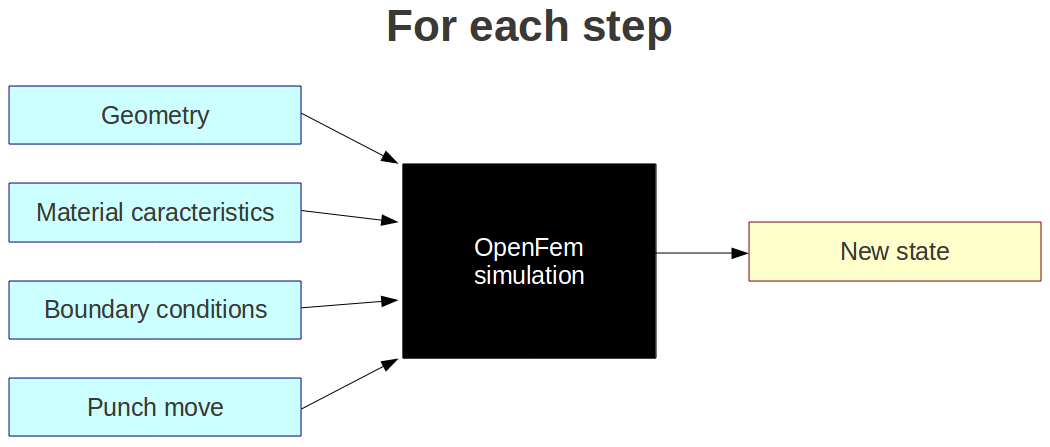
\includegraphics[width=\textwidth]{img/openFem.png}
        \caption{Dialog between Open fem and internal scene representation}
    \end{figure}
\end{frame}
\subsection{User interface}
\begin{frame}
    In a one operation cycle we will allow the user to:
    \begin{itemize}
        \item Define the system's initial state.
        \item Indicate the simulation's parameters.
        \item Visualize all the simulation steps.
        \item Visualize the trajectories of the free parts of the metal sheet.
        \item Visualize the distance between two points at a given step.
        \item Follow a given point over the time.
    \end{itemize}
\end{frame}
\begin{frame}
    \begin{figure}
        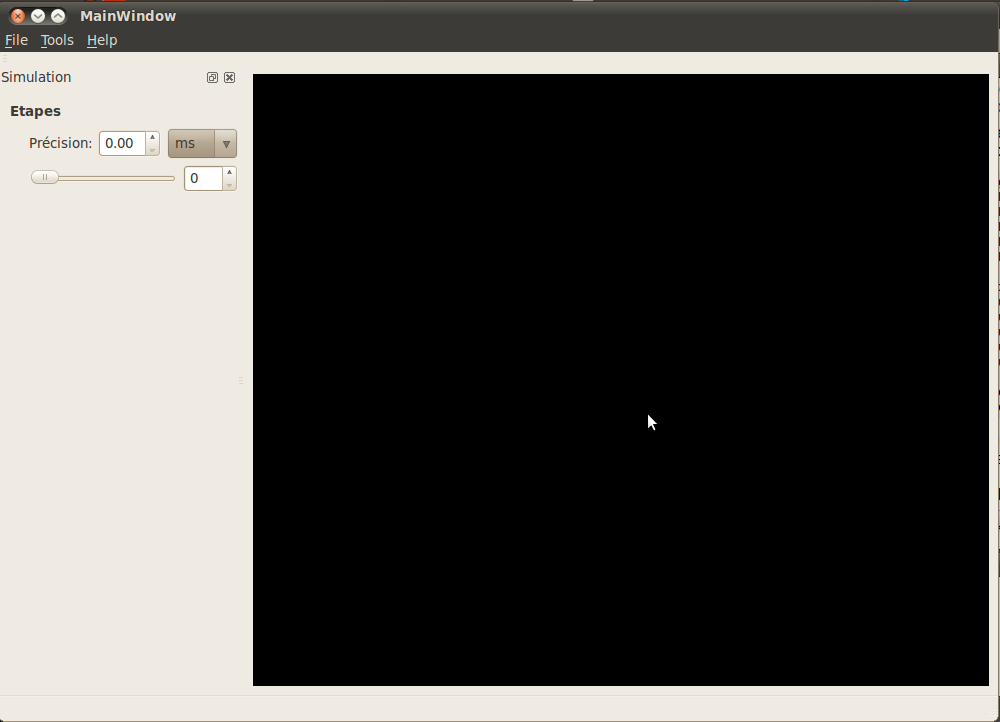
\includegraphics[width=\textwidth]{img/interface.png}
        \caption{The graphical user interface}
    \end{figure}
\end{frame}
\subsection{Implementation model}
\section{Tasks and progress}
\subsection{Gantt diagram}
\begin{frame}
    \begin{figure}
        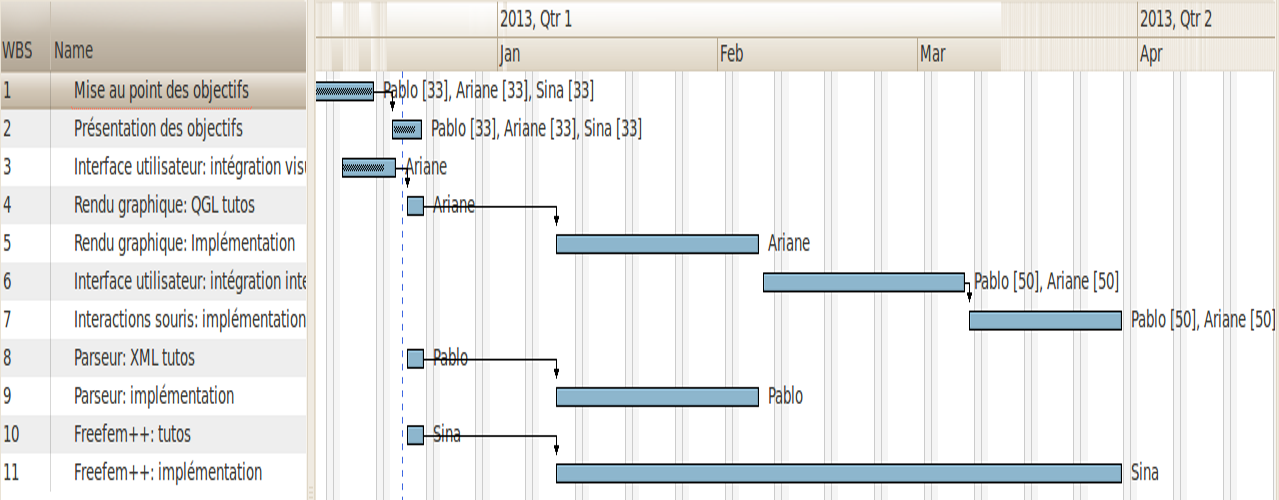
\includegraphics[width=\textwidth]{img/gantt.png}
        \caption{Gantt Diagram}
        \label{DiagrammeDeGant}
    \end{figure}
\end{frame}
\subsection{Tasks repartition}
\begin{frame}
    \begin{itemize}
        \item MCS: handles open fem\\
            Compute the metal sheet's deformation at every step.
        \item ICAO: visual rendering.\\
            Graphical user interface and interaction.
        \item ICAO: XML scene description and parser.\\
            Communication with open fem.
    \end{itemize}
\end{frame}
\begin{frame}
    \begin{figure}
        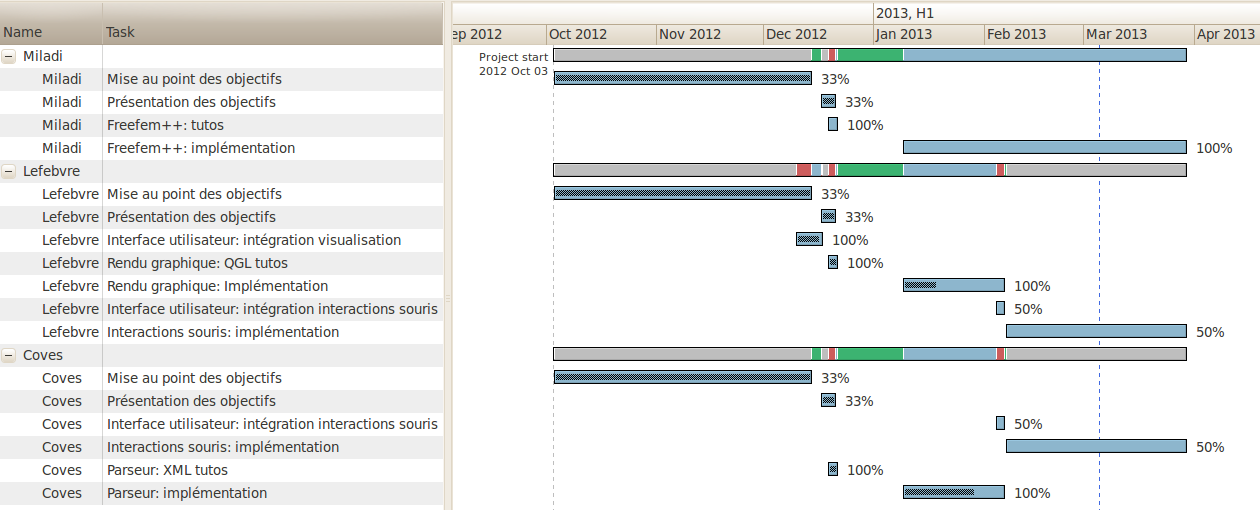
\includegraphics[width=\textwidth]{img/ganttRepartition.png}
        \caption{Tasks repartition}
        \label{Répartition}
    \end{figure}
\end{frame}
\subsection{Tasks completion}
\begin{frame}
    \begin{figure}
        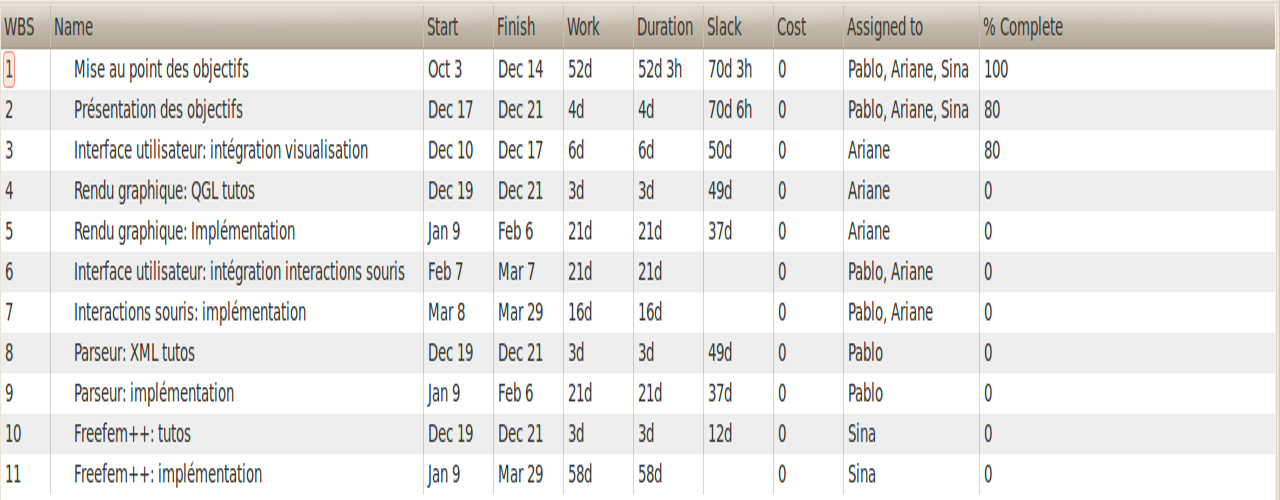
\includegraphics[width=\textwidth]{img/ganttCompletionTasks.png}
        \caption{Tasks completion}
        \label{Complétion}
    \end{figure}
\end{frame}

\section{Conclusion}
\subsection{Possibilities}
\begin{frame}
    \begin{itemize}
        \item Take sheet metal thickness modification into account.
        \item Evaluate spring back compensation to modify punch and die geometries.
    \end{itemize}
\end{frame}
\subsection{Questions}
\begin{frame}
    Thank you for your attention.
    \hfill Any questions?
\end{frame}

\end{document}
